\documentclass[fleqn, a4paper, 1pt]{article}       %fleqn => flushleft equation, setzte alle Formeln linksbündig
\usepackage[ngerman]{babel}
\usepackage[utf8]{inputenc}
\usepackage[official]{eurosym}
\usepackage{amsmath}
\usepackage[onehalfspacing]{setspace}
\usepackage{booktabs}
\usepackage{siunitx}
\sisetup{locale=DE}
\sisetup{per-mode=fraction}
\usepackage{graphicx}
\usepackage{pdfpages}
\usepackage{wrapfig}
\usepackage{subfigure}
\usepackage[toc,page]{appendix}

%Für Zitate
\usepackage[backend=biber,style=alphabetic]{biblatex}   %evtl immer mal wieder <biber Kurzbericht_ELK1_arndt-karger.bcf > laufen lassen; \cite{tl084}

\addbibresource{literatur.bib}


\begin{document}

\begin{titlepage}
	\centering
	%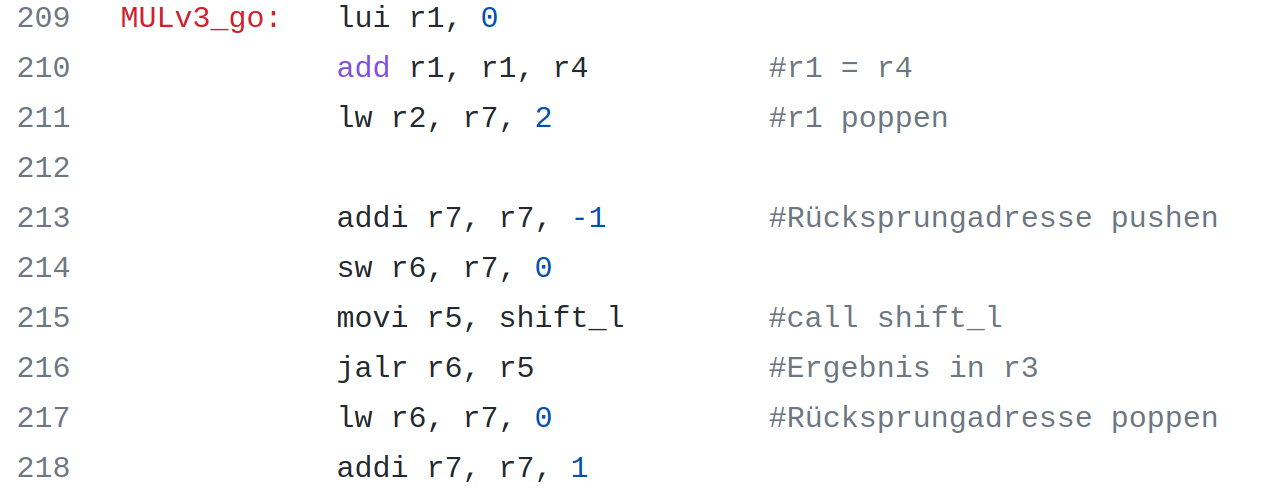
\includegraphics[width=0.8\textwidth]{Titelbild.png}\par\vspace{1cm}
	{\scshape\LARGE Technische Hochschule Mittelhessen \par}
	\vspace{1cm}
	{\huge\bfseries Dokumentation der Projektarbeit \par}
	\vspace{1.5cm}
	{\scshape\Large Systemroutinen für einen RiSC16 Prozessor \par}
	\vspace{2cm}
	{\Large\itshape vorgelegt von: \\ Arndt Karger \\ Elektro-  und Informationstechnik\\ Matr.Nr. 5317057\par}
	\vfill
	beleitet durch\par
    Prof. Dr.-Ing. Werner Bonath
	\vfill

% Bottom of the page
	{\large Gießen, \today\par}
\end{titlepage}

\thispagestyle{empty}
{\huge\bfseries Selbstständigkeitserklärung \par}
\vspace{1cm}

\noindent Ich versichere, dass ich die vorliegende Arbeit selbstständig verfasst und keine anderen als die angegebenen
Quellen und Hilfsmittel benutzt habe. Die Arbeit hat in gleicher oder ähnlicher Form noch keiner anderen
Hochschule oder Prüfungsstelle vorgelegen.

\vspace{4cm}
\begin{flushleft}
\begin{tabular}{@{}l@{}}\hline
Ort, Datum, Unterschrift
\end{tabular}
\end{flushleft}

\newpage
\thispagestyle{empty}
\tableofcontents
\newpage
\setcounter{page}{1}

\section{Einleitung}
Bei dem vorliegenden RiSC16 Prozessor handelt es sich um eine der MIPS Architektur (Microprocessor without interlocked pipeline stages) \cite{MIPS} ähnliche Architektur, welche über einen 16 Bit Adressraum, acht Register und acht Befehle verfügt. Desweiteren stehen ein Assembler von B. Jacob, ein Simulator sowie eine Hardwareimplementierung als FPGA von Prof. Dr.-Ing. W. Bonath zur Verfügung.

Der Befehlssatz gliedert sich in zwei Befehle zur Addition (addiere Register mit Register, addiere Register mit Ganzzahl), zwei Befehle für den Speicherzugriff (speichern und laden), einen Logikbefehl (\emph{nand}), einen Befehl zum laden der oberen zehn Bits einer Ganzzahl (\emph{lui}), sowie zwei Sprungbefehlen (bedingter Sprung, Sprung zu Adresse) auf. Zusatzlich zu diesen acht Befehlen stehen im Assembler zwei Makros zur Verfügung. Das eine (\emph{movi}) lädt die Adresse eines Markers in ein Register, das andere (\emph{halt} $\widehat{=}$ \emph{jalr r0, r0}) stoppt den Programmablauf. Von den acht bereitgestellten Registern sind sieben frei verwendbar. Das erste Register (r0) beinhaltet immer den Wert $0000_{hex}$.

Vor Beginn der eigentlichen Projektarbeit wurde die Dokumentation von B. Jacob gesichtet, sowie die von ihm zur Verfügung gestellten Testprogramme ausgeführt.


\section{Aufgabenstellung}
Ziel dieser Projektarbeit war das Schreiben von Systemroutinen in Assembler, um die Funktion des Prozessors zu veranschaulichen, sowie die Hardwareimplementierung zu testen. Es sollte deutlich gemacht werden, dass auch mit dem einfachen Befehlssatz komplexe Probleme gelöst werden können. Dies wurde hier beispielhaft an zwei möglichen Multiplikationsalgorithmen durchgeführt. Die beiden Algorithmen sind die Multiplikation via Addition und eine bitweise Multiplikation. Zuerst wurde ein Stack in Software implementiert, um das Sichern von Registern beim Aufruf der Routinen möglich zu machen. Dann wurde für die Multiplikation via Addition ein Flussdiagramm erstellt und in Assembler implementiert. Nach einer kurzen Literaturrecherche über die genaue Funktion der bitweisen Multiplikation wurde auch hierfür ein Flussdiagramm erstellt und schließlich implementiert. Der Code wurde während der Entwicklungsphase in dem von Herrn Prof. Dr.-Ing. Bonath entwickelten Simulator fortlaufend getestet und mit Git getrackt.

\section{Erstellte Routinen}
\subsection{Stackoperationen}

Die RiSC16 Architektur verfügt über keinerlei Stackoperationen. Daher wird beim Programmstart ein Stack in Software initialisiert. Das Register r7 dient hierbei als Stackpointer (SP). Dieses wird zuerst mit der Startadresse des Stack (hier $7FFF_{hex}$) beschrieben. Dieses Date steht hart im Speicher und wird über den Marker \glqq Stack\_adr\grqq \ abgerufen (vergleiche (vgl.) Abbildung (Abb.) \ref{fig:Stack}).
Der Stack wurde  \glqq Bottom-Up\grqq \ implementiert, was bedeutet, dass er zu kleiner werdenden Adressen hin wächst (von unten nach oben). Das Register r7 zeigt immer auf den Top-Of-Stack (TOS), die Grenzen des Stack werden nicht überwacht.

Man erreicht die Funktion \emph{push}  durch einmaliges dekrementieren des SP und speichern eines Registers mit dem Befehl \emph{sw} (store word) (vgl. Abb. \ref{fig:Stack} line 12 folgende). Analog \emph{pop} durch laden eines Dates aus dem Speicher via \emph{lw} (load word) und anschließendem inkrementieren des SP. Eine indirekte Adressierung ist mittels eines Immediate-Offsets möglich (vgl. Abb. \ref{fig:Stack} line 14).

Prinzipiell ist das ausreichend um mit dem Stack arbeiten zu können. Um eine größere Lesbarkeit beim debuggen zu schaffen, werden in der Initialsierung auch noch der Anfang sowie das Ende des Stacks markiert. Dazu wird in das Register r1 das Date $-1_{dez}\ \widehat{=}\ FFFF_{hex}$ geschrieben und an die erste und letzte Adresse im Stack gepusht (vgl. Abb. \ref{fig:Stack} line 11 fort folgende).

\begin{figure}[h]
    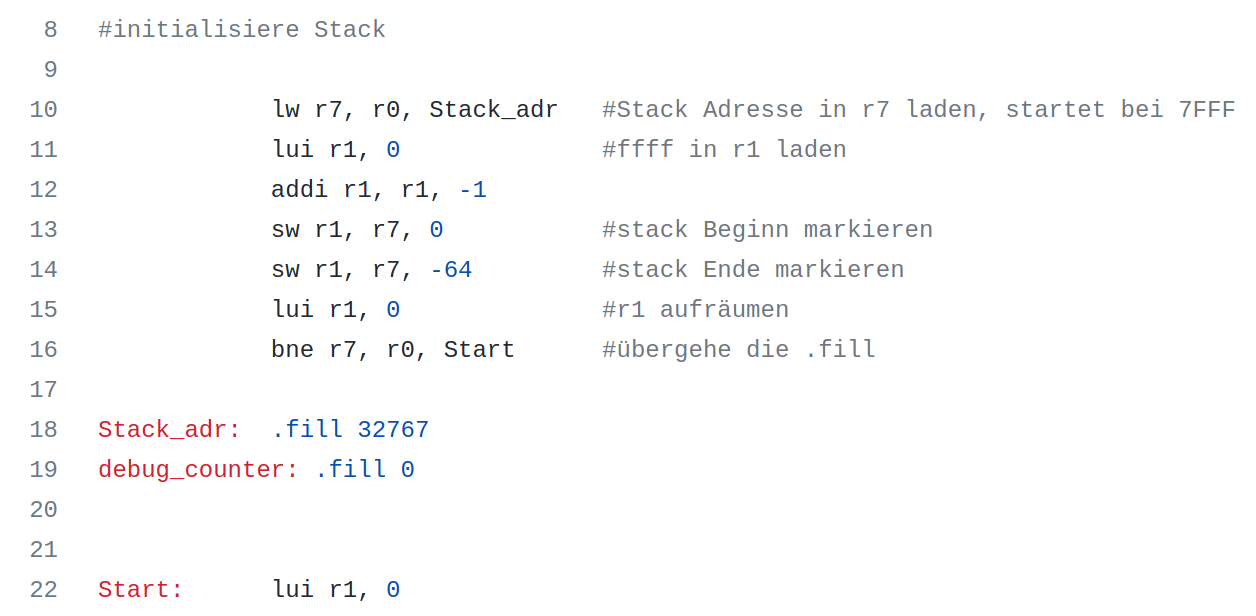
\includegraphics[width =1\textwidth]{Stack_init.png}
\caption{Initialisierung des Stack}
\label{fig:Stack}
\end{figure}



\subsection{Multiplikation via Addition}
Eine Möglichkeit eine Multiplikation zu implementieren besteht darin den Multiplikanten so oft zu sich selbst dazu zu addieren, wie es der Multiplikator vorschreibt. Aus $X = 3 \cdot 3$ wird also $X = 3+3+3$. Diese Art der Multiplikation ist sehr einfach durch eine Schleife zu realisieren und wurde in der Routine \emph{MULv2} angewendet. Hierbei wird der Multiplikant (r2) solange auf das Ergebnisregister (r3) addiert, bis der Multiplikator zu Null geworden ist. 

\subsection{Bitweise Multiplikation}
Eine andere Möglichkeit der Multiplikation besteht darin, zwei Zahlen bitweise zu multiplizieren. Der entwickelte Multiplikationsalgorithmus funktioniert nach folgendem Prinzip: 

Betrachten wir beispielhaft die Multiplikation von zwei Acht-Bit-Zahlen \\ ($n = 8$), eine ist der Multiplikant, die andere der Multiplikator. Zuerst untersuchen wir das Most Significant Bit (MSB) des Multiplikators, also das siebte Bit. Ist dieses gesetzt, so schieben wir den Multiplikanten um die Wertigkeit des untersuchten Bits (hier sieben) nach links und addieren das auf das Ergebnisregister. Ist es nicht gesetzt, so geschieht nichts. \cite{MULv3}

Analog verfahren wir mit allen weiteren Bits. Diesen Prozess müssen wir für alle Bits des Multiplikators durchführen, in unserem Beispiel ergibt das acht Wiederholungen (vgl. Abb. \ref{fig:bitw_Mul_Prinzip}). Dieser Prozess ist unabhängig von der Bitbreite.



\begin{figure}[h]
    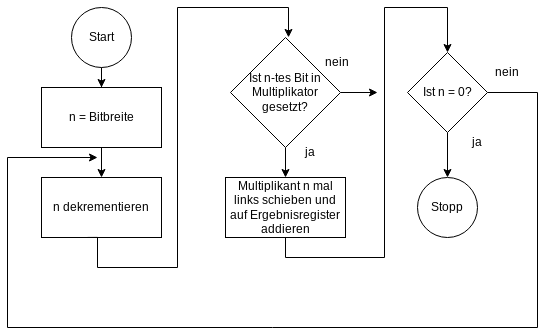
\includegraphics[width =1\textwidth]{bitweise_Mul_Prinzip.png}
\caption{Funktionsprinzip des bitweise Multiplizierers}
\label{fig:bitw_Mul_Prinzip}
\end{figure}



Da die RiSC16 Architektur über keinerlei Schiebebefehle verfügt, wurde hierfür ein kleines Unterprogramm entworfen, welches als Rückgabewert das um eine gewünschte Schrittweite geschobenes Register hat und nach folgendem Prinzip arbeitet:

Im einfachen Binärsystem hat die Stelle $n+1$ immer genau die doppelte Wertigkeit der Stelle $n$. Bsp.: $2^2 = 4 = 2 \cdot 2^1$. Schiebt man also ein Wort nach links und füllt rechts mit Nullen auf, so verdoppelt sich die Wertigkeit des Wortes mit jedem Schiebevorgang, kommt also einer Multiplikation mit zwei gleich. Bei einer gewünschten Schrittweite $m$ verdoppelt dieses Unterprogramm das Register also $m$-mal.


\section{Zusammenfassung}

\begin{itemize}
    \item Vor- und Nachteile der einzelnen Algorithmen
\end{itemize}




% \section{Verwendete Abkürzungen}
% \subsection{Allgemeine Abkürzungen}
% \begin{itemize}
%     \item Abb. : Abbildung
%     \item Bsp. : Beispiel
%     \item f. : folgende. Bsp.: line 12f. bedeutet line 12 und 13
%     \item ff. : fortfolgende. Bsp.: line 12ff. bedeutet line 12 bis zum Ende des Blocks
%     \item Vgl. : vergleiche
% \end{itemize}
%
% \subsection{Technische Abkürzungen}
% \begin{itemize}
%    % \item LSB : Least Significant Bit
%     \item MSB : Most Significant Bit
%     \item SP : Stackpointer
%     \item TOS : Top-Of-Stack
% \end{itemize}

\newpage
\appendix %sagt ab hier ist Anhang
\section{Anhang}
\subsection{Verwendung der entworfenen Routinen}

\begin{figure}[h]
    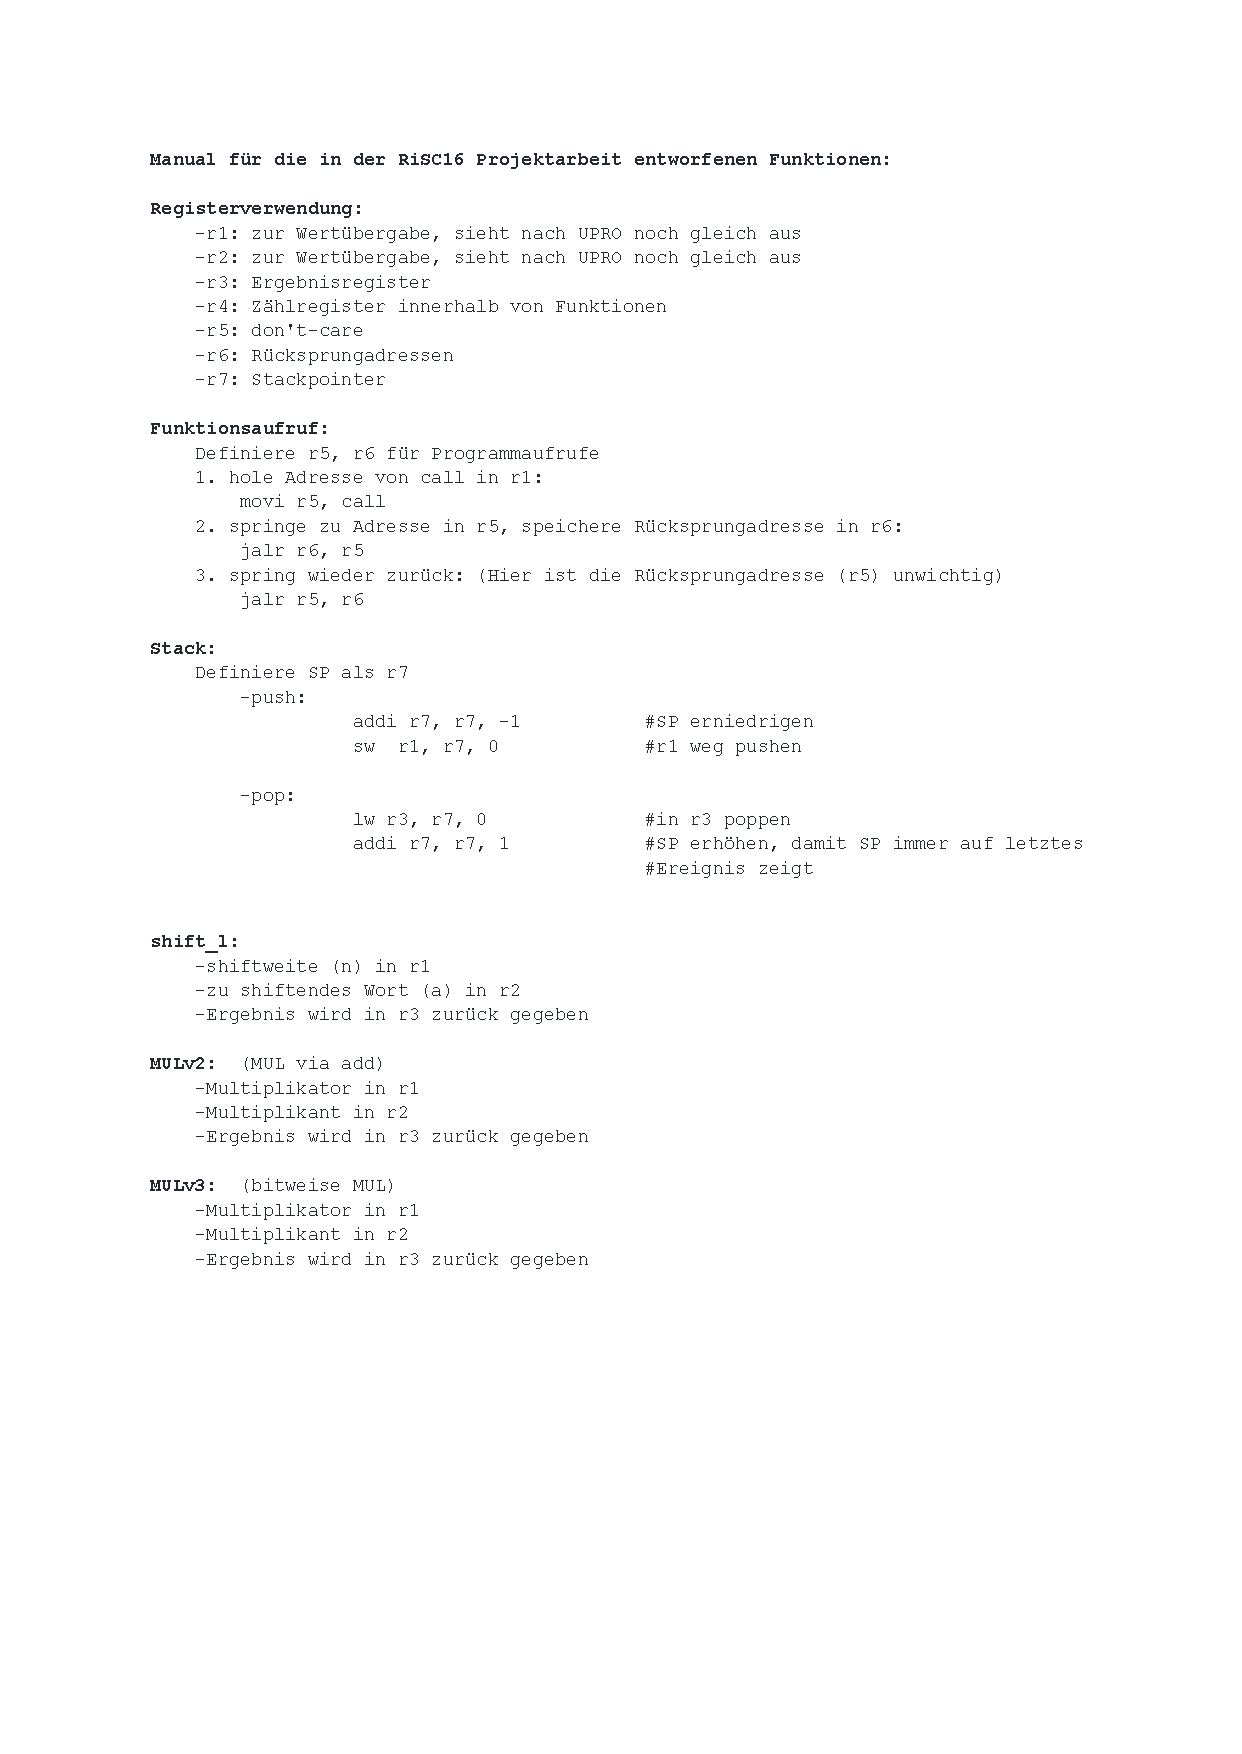
\includegraphics[width =1\textwidth]{Manual.png}
%\caption{Funktionsprinzip des bitweise Multiplizierers}
\label{fig:bitw_Mul_Prinzip}
\end{figure}

\newpage

\subsection{Multiplikation via Addition: (MULv2)}
Funktionalität:

Multipliziere zwei vorzeichenlose Zahlen.
\\

\noindent Verwendung:
\begin{itemize}
	\item $r3 = r1 \cdot r2$
	\item Multiplikator und Multiplikant vor Programmaufruf  in r1                und r2 laden.
	\item Diese stehen auch nach Programmablauf unverändert                dort.
\end{itemize}

\begin{figure}[h]
    \centering
    \includegraphics[width =0.55\textwidth]{Mulv2.png}
\caption{Flussdiagramm MULv2}
\label{fig:bitw_Mul_Prinzip}
\end{figure}

\newpage

\subsection{Bitweise Multiplikation: (MULv3)}
Funktionalität:

Multipliziere zwei vorzeichenbehaftete Acht-Bit-Zahlen
\\

\noindent Verwendung:
\begin{itemize}
	\item $r3 = r1 \cdot r2$
	\item Multiplikator und Multiplikant vor Programmaufruf in r1 und r2 laden.
	\item Diese stehen auch nach Programmablauf unverändert                dort.
\end{itemize}
\vspace{4cm}
\begin{figure}[h]
    \centering
    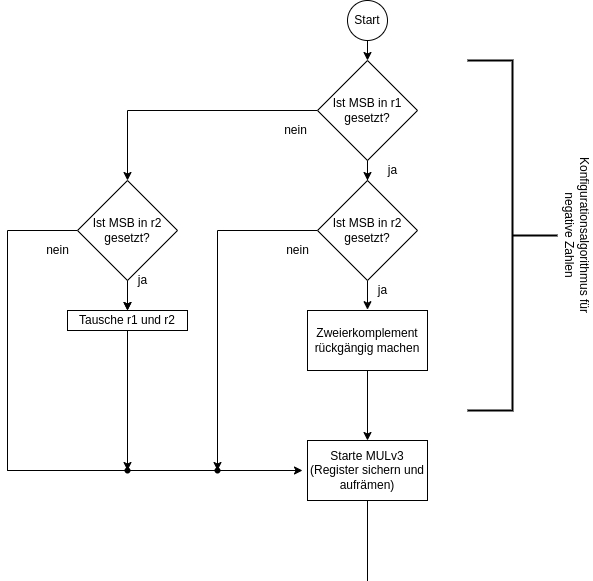
\includegraphics[width =0.55\textwidth]{MULv3-1.png}
%\caption{Flussdiagramm MULv2}
\label{fig:bitw_Mul_Prinzip}
\end{figure}

\newpage

\begin{figure}[h]
    \centering
    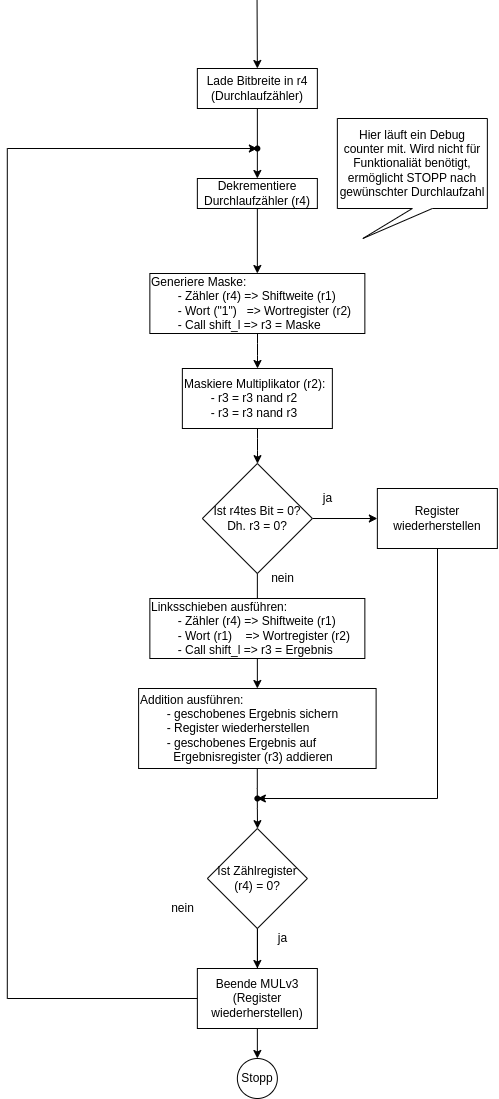
\includegraphics[width =0.55\textwidth]{MULv3-2.png}
\caption{Flussdiagramm MULv3}
\label{fig:bitw_Mul_Prinzip}
\end{figure}


%




\newpage
\printbibliography  % so werden Zitate angegeben: \cite{name}
\addcontentsline{toc}{section}{Literaturverzeichnis}






















\end{document}

